%!TEX root = ../thesis.tex
% **************************** Define Graphics Path **************************
\ifpdf
\graphicspath{{Chapter5/Figs/Raster/}{Chapter5/Figs/PDF/}{Chapter5/Figs/}}
\else
\graphicspath{{Chapter5/Figs/Vector/}{Chapter5/Figs/}}
\fi

%*******************************************************************************
%****************************** Fifth Chapter *********************************
%*******************************************************************************

\chapter{Experiments and Results}
\label{chapter5}

\section{Stoquastic lattice models}

\subsection{Transverse-field Ising model}
\label{sec:res-im}
If we transform the transverse-field Ising model Hamiltonian in eq.\eqref{eq:ising_hamiltonian} into the $z$-spin basis, where $s = $
\begin{figure}[h]
	\centering
	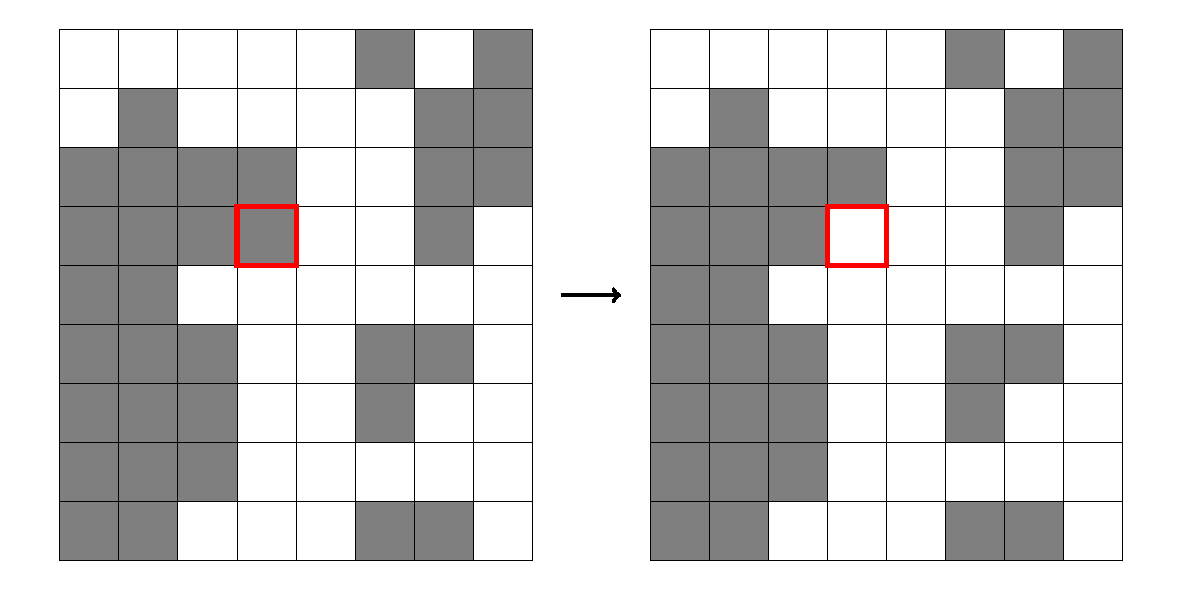
\includegraphics[width=0.7\linewidth]{Chapter6/Figs/Vector/ising_passive}
	\caption[Ising passive process]{\textbf{Ising passive process}}	
	\label{fig:isingpassive}
\end{figure}
\subsection{Heisenberg model}
\label{sec:res-hm}
\begin{figure}[h]
	\centering
	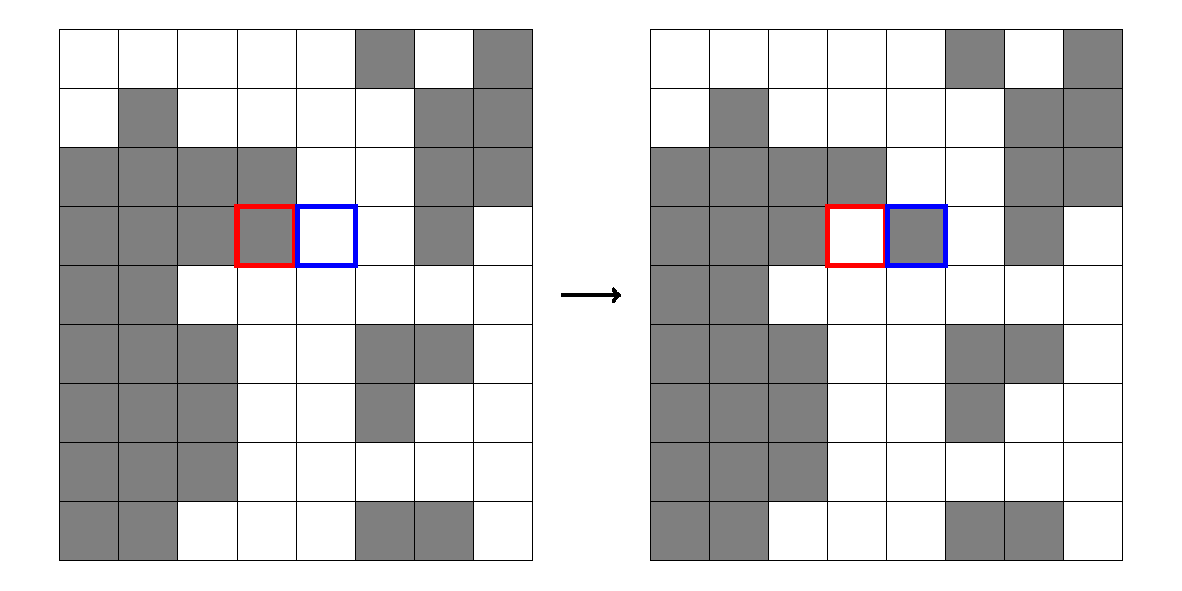
\includegraphics[width=0.7\linewidth]{Chapter6/Figs/Vector/xy_passive}
	\caption[XY passive process]{\textbf{XY passive process}}
	\label{fig:xypassive}
\end{figure}

Heisenberg ferromagnet
\begin{equation}
\hat H_{\mathrm{F}}=-\frac{1}{2} \sum_{j}\left[\hat{\sigma}_{j}^{x} \hat{\sigma}_{j+1}^{x}+\hat{\sigma}_{j}^{y} \hat{\sigma}_{j+1}^{y}+\hat{\sigma}_{j}^{z} \hat{\sigma}_{j+1}^{z}\right]
\end{equation}

The XY model.
\begin{equation}
\begin{aligned} 
\hat H_{X Y}=-\sum_{j}\left[\hat{\sigma}_{j}^{x} \hat{\sigma}_{j+1}^{x}+\hat{\sigma}_{j}^{y} \hat{\sigma}_{j+1}^{y}\right] &=H_{\mathrm{F}}+\frac{1}{2} \sum_{j} \hat{\sigma}_{j}^{z} \hat{\sigma}_{j+1}^{z} \\ 						&=-\mathcal{W}+\sum_{j}\left[n_{j}\left(1-n_{j+1}\right)+n_{j+1}\left(1-n_{j}\right)\right] 
\end{aligned}
\end{equation}

\begin{equation}
\psi_{s_{1: N}}(t)=\underset{\Sigma_{[0, t]} \sim \operatorname{SEP} \text{ with } \Sigma_{t}=s_{1: N}}{\mathbb{E}}
\left[\exp \left(-\int_{0}^{t} d t^{\prime} \sum_{j}\left[n_{j}\left(1-n_{j+1}\right)+n_{j+1}\left(1-n_{j}\right)\right]\right) \psi_{\Sigma_{0}}(0)\right]
\end{equation}

%\subsection{Bose-Hubbard model}
%\label{sec:res-bhm}

\section{Learning the rates} 
\begin{figure}
	\centering
	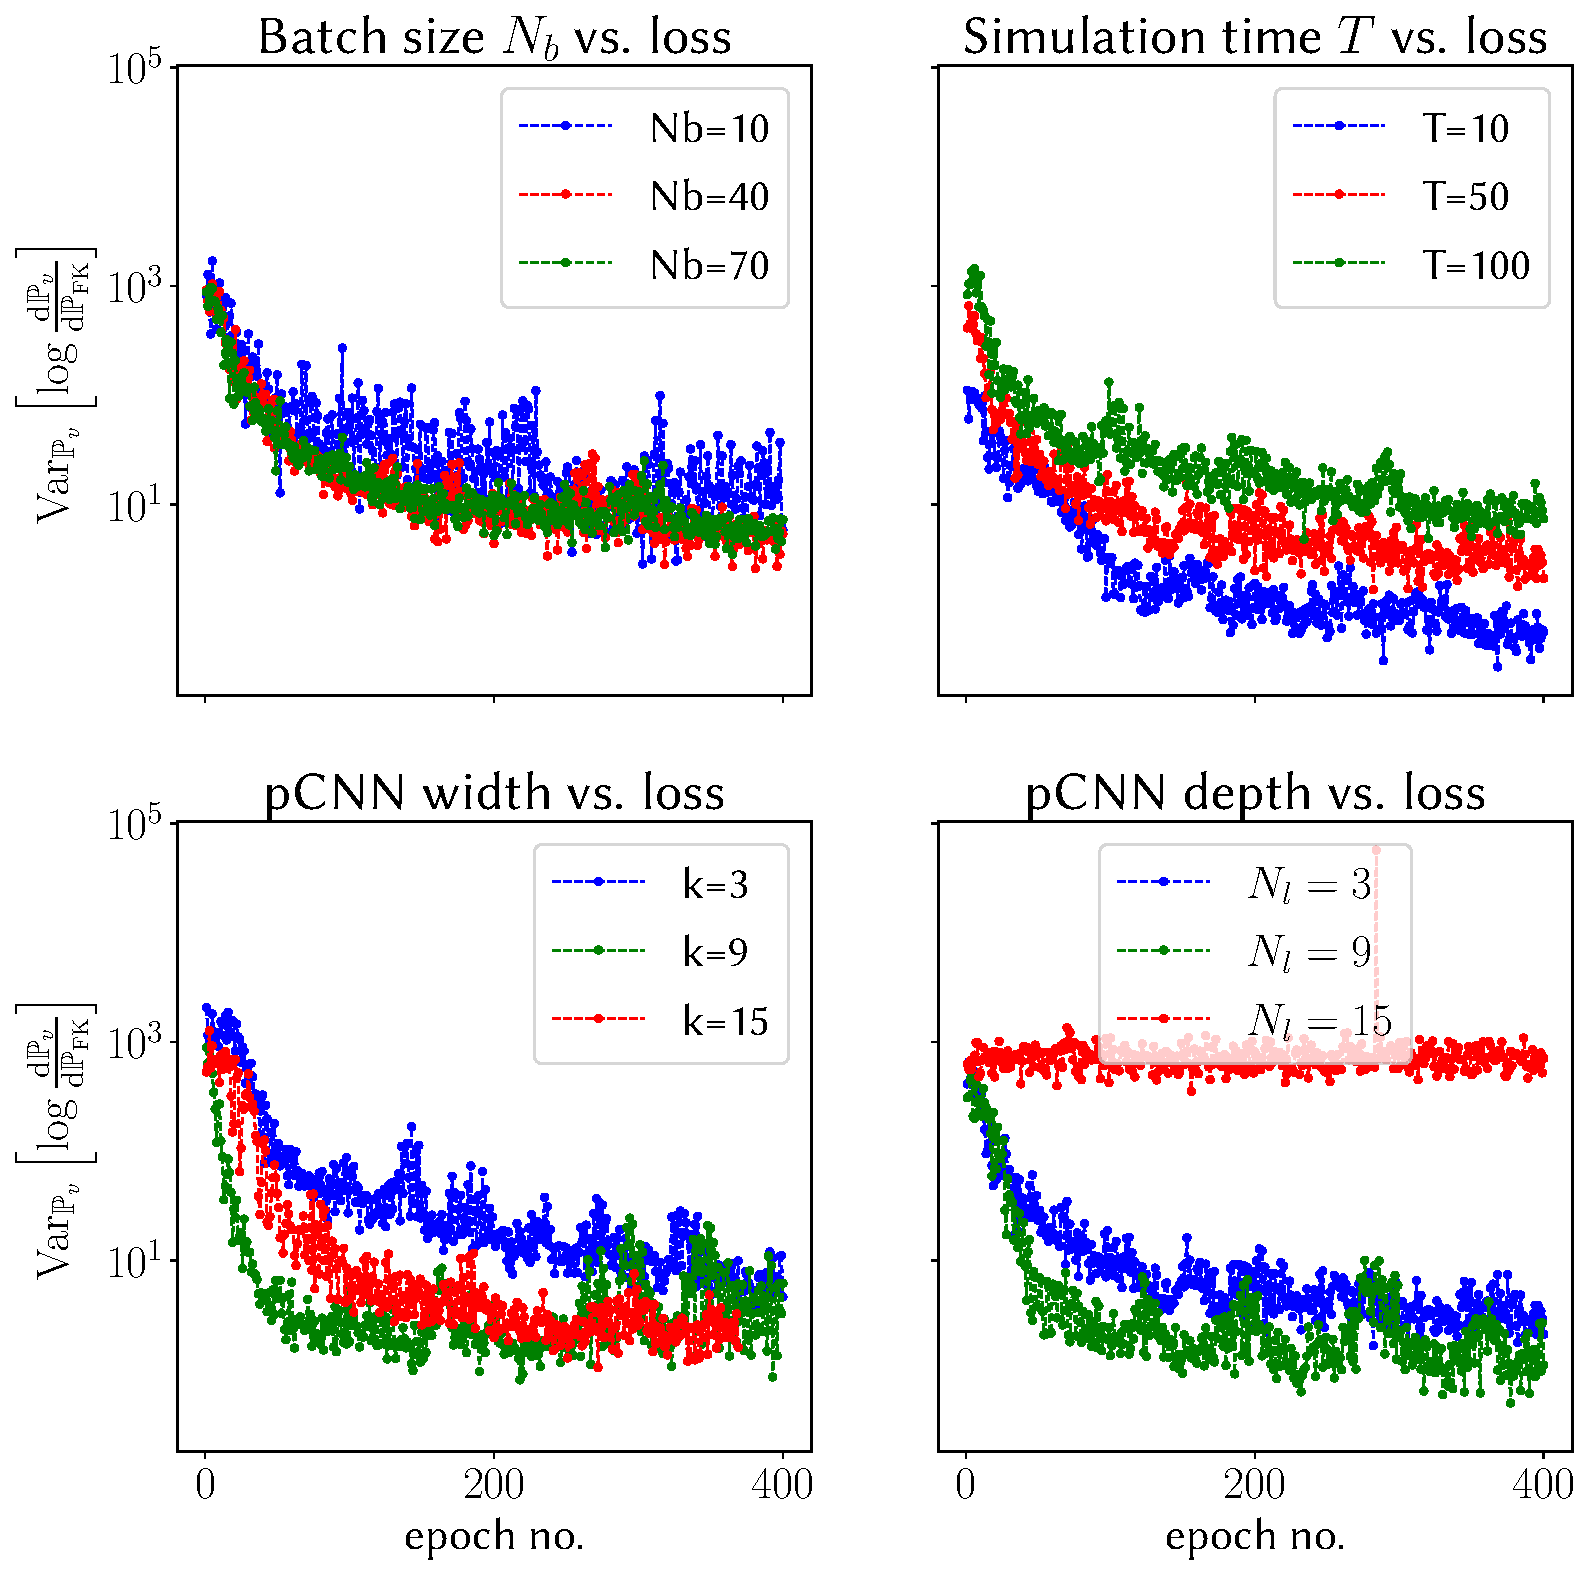
\includegraphics[width=\linewidth]{Chapter5/Figs/Vector/init_test_learning}
	\caption[Initial rate training experiments]{\textbf{Initial rate training experiments}}
	\label{fig:inittestlearning}
\end{figure}

\subsubsection{How does simulation time $T$ and batch size $N_b$ affect the learning of the rates?}

\subsubsection{How do architectural choices of the pCNN limit learning the rates?}

\subsubsection{How does the size of lattice play a role?}

\subsubsection{Can we improve learning by scaling the output of the pCNN?}
Also mention reshuffling.

\subsubsection{What role does symmetry play in all of this?}

\section{Importance sampling}

\subsection{Ising model}

\subsection{XY model}

%\begin{figure}[H]
%	\centering
%	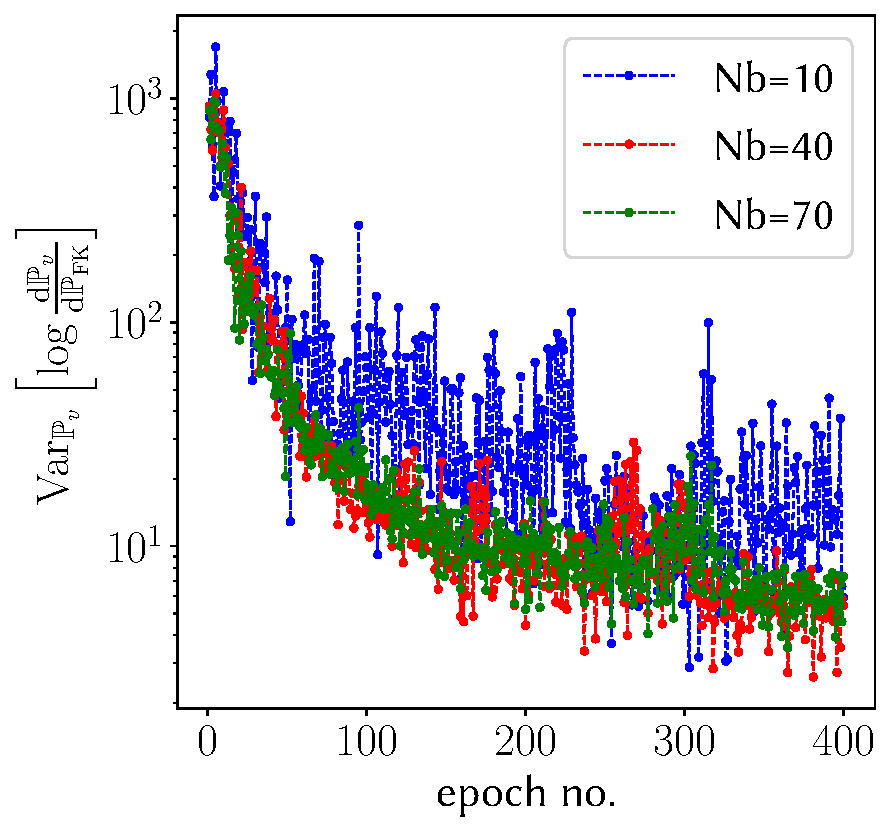
\includegraphics[width=\linewidth]{Chapter6/Figs/Vector/bvl_single}
%	\caption[Effect of batch size $N_b$ on training with the endpoint loss.]{\textbf{Effect of batch size $N_b$ on training with the endpoint loss.}}
%	\label{fig:bvlsingle}
%\end{figure}
%\begin{figure}[H]
%	\centering
%	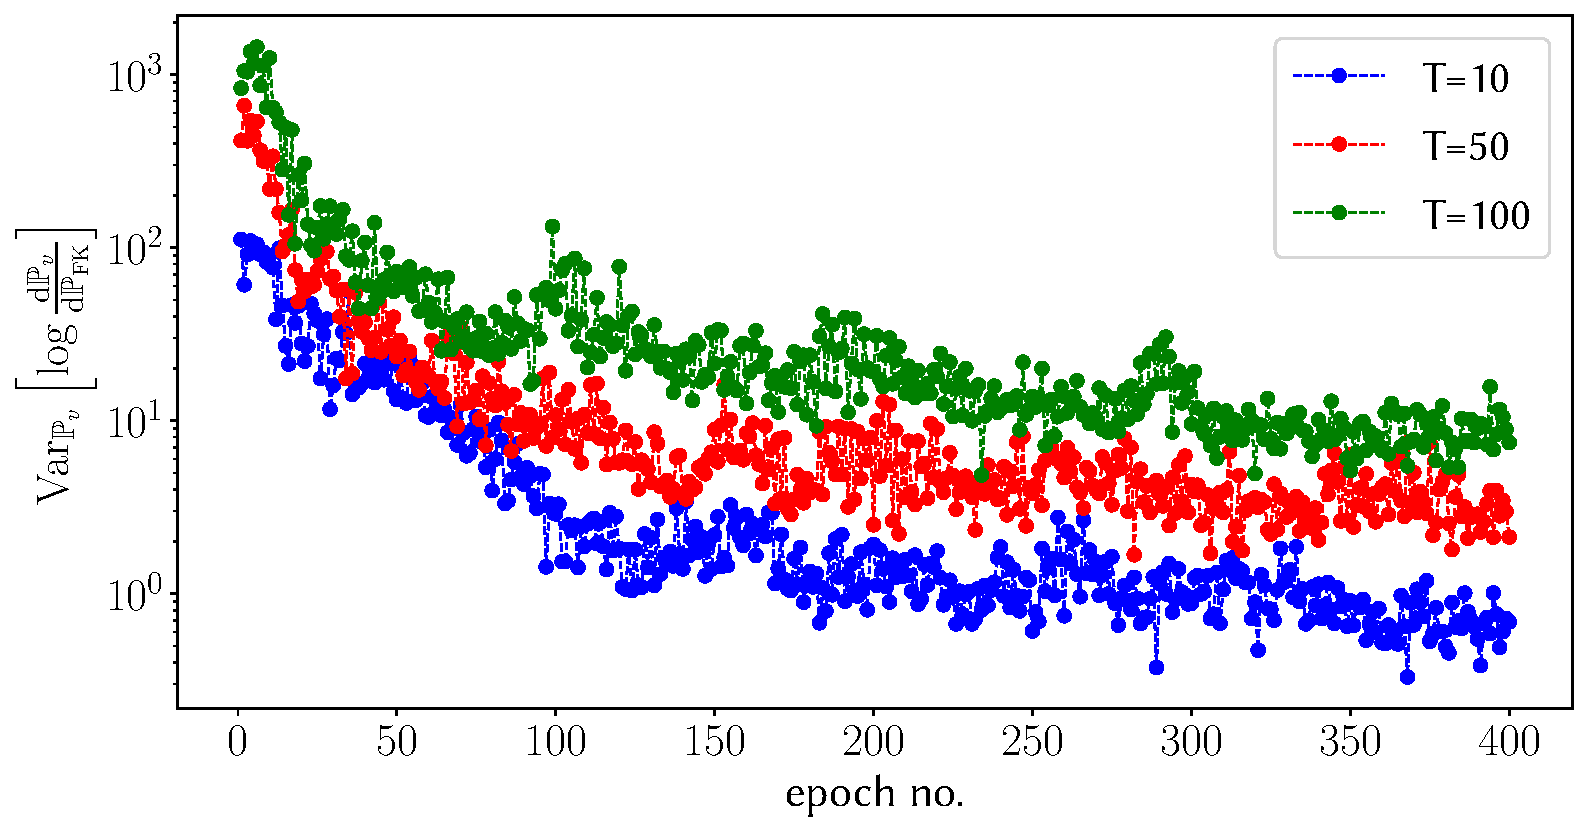
\includegraphics[width=\linewidth]{Chapter6/Figs/Vector/tvl_single}
%	\caption[Effect of simulation time $T$ on training with the endpoint loss.]{\textbf{Effect of simulation time $T$ on training with the endpoint loss.}}
%	\label{fig:tvlsingle}
%\end{figure}
%\begin{figure}[H]
%	\centering
%	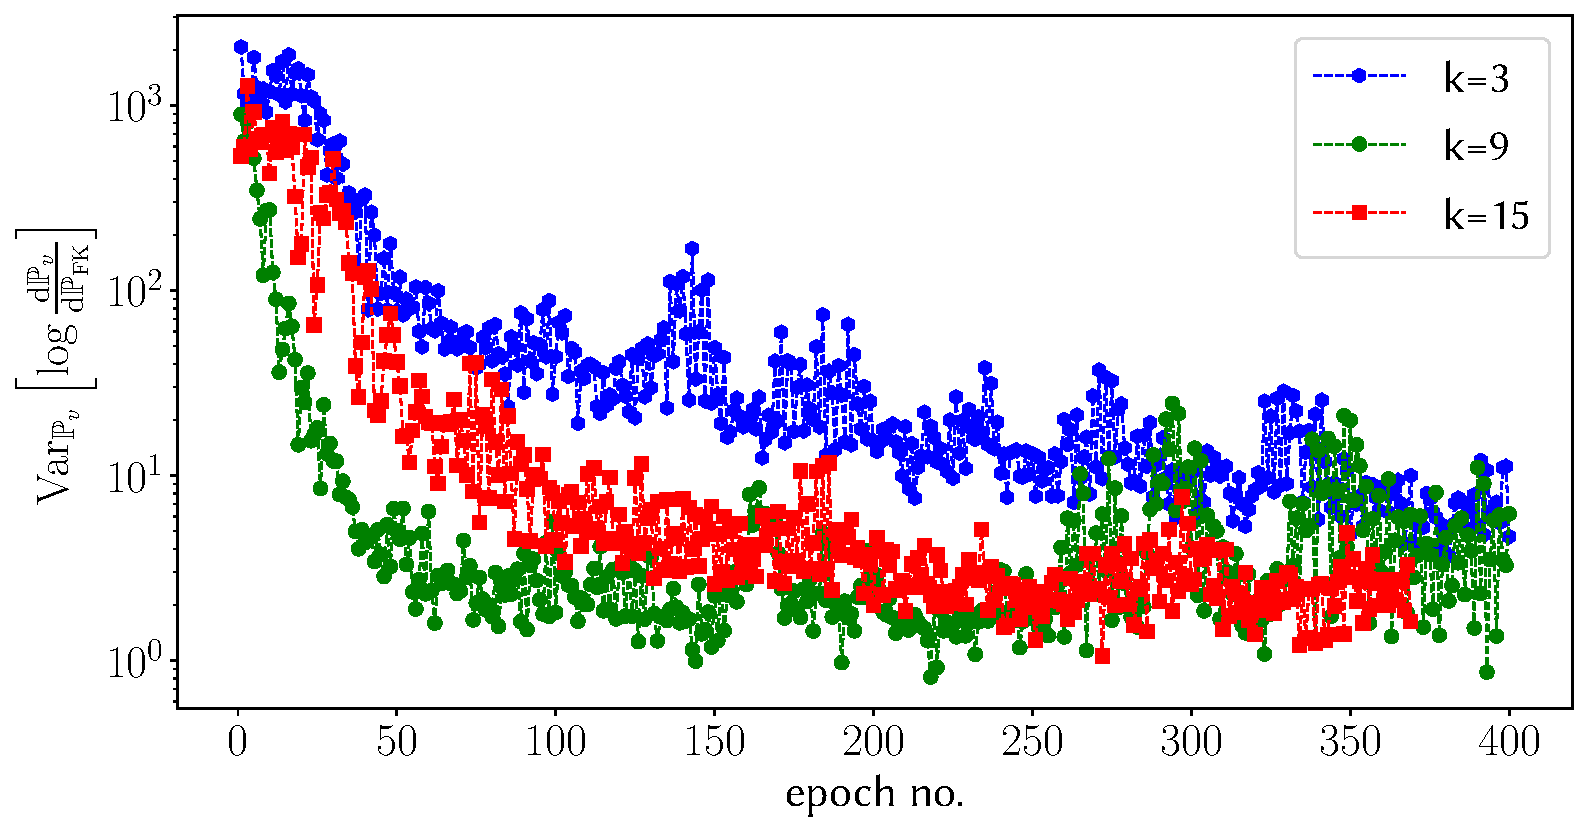
\includegraphics[width=\linewidth]{Chapter6/Figs/Vector/wvl_single}
%	\caption[Effect of pCNN width $k$ on training with the endpoint loss.]{\textbf{Effect of pCNN width $k$ on training with the endpoint loss.}}
%	\label{fig:wvlsingle}
%\end{figure}
%\begin{figure}[H]
%	\centering
%	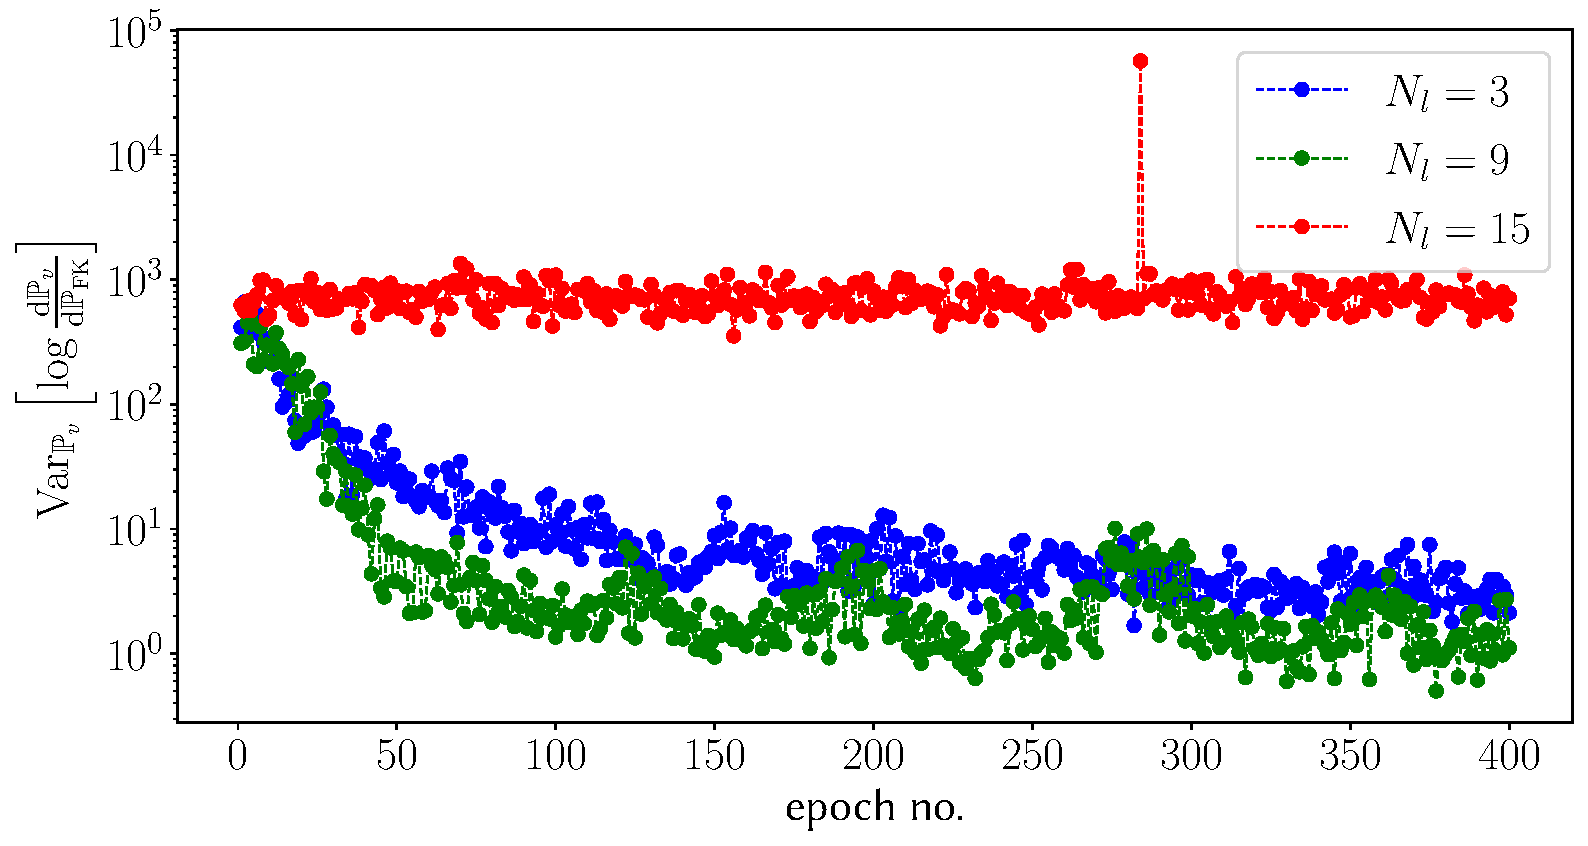
\includegraphics[width=\linewidth]{Chapter6/Figs/Vector/lvl_single}
%	\caption[Effect of pCNN depth $l$ on training with the endpoint loss.]{\textbf{Effect of pCNN depth $l$ on training with the endpoint loss.}}
%	\label{fig:lvlsingle}
%\end{figure}